% !TeX TS-program = txs:///latexmk | txs:///view-log | txs:///view-pdf | txs:///convert
\documentclass{article}

\usepackage{tikzducks}
\usepackage[paperwidth=38cm,paperheight=42cm,margin=1cm]{geometry}

\usepackage{bbding}

\newcommand{\addwizzard}{
	\path[fill=BlueViolet!50!Pink,line width=1pt,rotate=-5] 
	(52,190)--(92,290)--(132,190);
	\pgftext[at=\pgfpoint{71}{265}, left, base]{\color{Gold}\EightStarBold}
	\pgftext[at=\pgfpoint{63}{250}, left, base]{\color{Gold}\EightStarBold~\EightStarBold}
	\pgftext[at=\pgfpoint{56}{265}, left, base]{\color{Gold}\EightStarBold~\EightStarBold~\EightStarBold}
	\pgftext[at=\pgfpoint{56}{280}, left, base]{\color{Gold}\EightStarBold~\EightStarBold~\EightStarBold}
	\draw[line width=6pt,color=black] (90,90) -- (60,40);
	\draw[line width=6pt,color=white] (85,81.67) -- (80,73.33);
}

\newcommand{\addicecream}[3]{%
	\path[draw=Sienna,fill=Goldenrod,line width=1pt,rotate=-20] 
	(-5,140)--(10,80)--(25,140);
	\path[draw=Sienna, fill=Goldenrod, rotate=-20,line width=1pt] (94,82) ellipse (14.29 and 8.93);
	\path[fill=#1, rotate=-20] (88,64) circle (10.7);
	\path[fill=#2, rotate=-20] (98,84) circle (10.7);
	\path[fill=#3, rotate=-20] (92,98) circle (10.7);
}

\newcommand{\addbook}[2]{%
		\path[fill=#1,rotate=20] (110,130) rectangle (150,70);
		\node[rotate=-20, color=white] at (73,70)  {%
			\resizebox{1cm}{!}{#2}};
}

\newcommand{\addwater}[1]{%
	\draw [decorate,decoration=snake, line width=3pt, color=#1] (0,50) -- (100,50);
	\draw [decorate,decoration=snake, line width=3pt, color=#1] (180,50) -- (220,50);
	\draw [decorate,decoration=snake, line width=3pt, color=#1] (50,40) -- (150,40);
	\draw [decorate,decoration=snake, line width=3pt, color=#1] (110,20) -- (250,20);
	\draw [decorate,decoration=snake, line width=3pt, color=#1] (20,10) -- (70,10);
	\draw [decorate,decoration=snake, line width=3pt, color=#1] (60,0) -- (250,0);
}


\begin{document}

%% normal
%\begin{tikzpicture}[y=0.80pt, x=0.80pt]
%	\duck{Gold}
%\end{tikzpicture}
%
%% grumpy
%\begin{tikzpicture}[y=0.80pt, x=0.80pt]
%	\grumpyduck{Gold}
%\end{tikzpicture}
%
%% alien duck
%\begin{tikzpicture}[y=0.80pt, x=0.80pt]
%	\duck{Gold}
%	\addalien{LimeGreen}
%\end{tikzpicture}
%
% short hairs
%\begin{tikzpicture}[y=0.80pt, x=0.80pt]
%	\duck{Wheat}
%	\addtshirt{LightBlue!50!white}
%	\addjacket{LightSlateGrey}
%	\addshorthair{brown!50!Grey}
%\end{tikzpicture}
%
%Men in black
%\begin{tikzpicture}[y=0.80pt, x=0.80pt]
%	\grumpyduck{Wheat}
%	\addtshirt{white}
%	\addjacket{black}
%	\addtie{black}
%	\addhat{black}
%	\addsunglasses{black}{black}
%\end{tikzpicture}
%
%
%% ducklings
%\begin{tikzpicture}[y=0.80pt, x=0.80pt, scale=0.6]
%	\duck{Gold}
%	\begin{scope}[xshift=300pt, scale=.3, yshift=250pt]
%		\duck{Gold}
%	\end{scope}
%	\begin{scope}[xshift=180pt, scale=.3, yshift=150pt]
%		\duck{Gold}
%	\end{scope}
%	\begin{scope}[xshift=240pt, scale=.3, yshift=50pt]
%		\duck{Gold}
%	\end{scope}		
%\end{tikzpicture}
%
% samcarter
%\begin{tikzpicture}[y=0.80pt, x=0.80pt]
%	\duck{Wheat!95!red}
%	\addjacket{MidnightBlue}
%	\addlonghair{OrangeRed!50!Brown}
%\end{tikzpicture}

%% hair
%\begin{tikzpicture}[y=0.80pt, x=0.80pt]
%	\duck{Gold}
%	\addlonghair{SeaGreen}
%\end{tikzpicture}
%
% unicorn
%\begin{tikzpicture}[y=0.80pt, x=0.80pt]
%	\duck{Pink}
%	\addlonghair{MediumVioletRed}
%	\addunicorn{VioletRed}
%\end{tikzpicture}
%
% hat duck
%\begin{tikzpicture}[y=0.80pt, x=0.80pt]
%	\duck{Gold}
%	\addhat{SaddleBrown}
%\end{tikzpicture}
%
% sunglasses
%\begin{tikzpicture}[y=0.80pt, x=0.80pt]
%	\duck{Gold}
%	\addsunglasses{black!50!brown}{black}
%\end{tikzpicture}
%
% normal duck
%\begin{tikzpicture}[y=0.80pt, x=0.80pt]
%	\duck{Gold}
%\end{tikzpicture}
%
% blue duck
%\begin{tikzpicture}[y=0.80pt, x=0.80pt]
%	\duck{SteelBlue}
%\end{tikzpicture}
%
% Brazil colour duck for Paulo
%\begin{tikzpicture}[y=0.80pt, x=0.80pt]
%	\definecolor{brazilgreen}{RGB}{0,155,58}
%	\definecolor{brazilyellow}{RGB}{254,223,0}
%	\definecolor{brazilblue}{RGB}{0,39,118}
%	\duck{brazilyellow}
%	\addjacket{brazilblue}
%	\addshorthair{brazilgreen}
%\end{tikzpicture}

% icecream
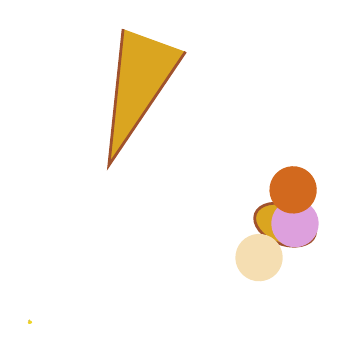
\begin{tikzpicture}[y=0.80pt, x=0.80pt]
	\duck{Gold}
	\addicecream{Wheat}{Plum}{Chocolate}
\end{tikzpicture}

% swimming
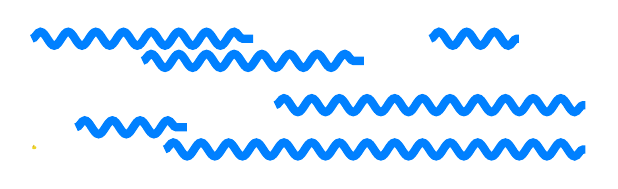
\begin{tikzpicture}[y=0.80pt, x=0.80pt]
	\duck{Gold}
	\addwater{blue!50!cyan} 
\end{tikzpicture}

% prof. van duck
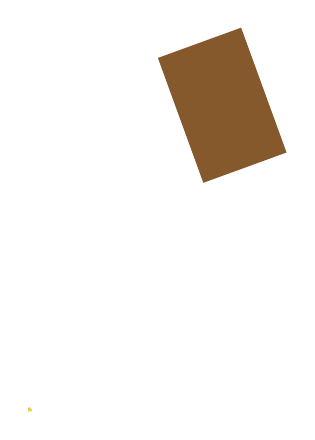
\begin{tikzpicture}[y=0.80pt, x=0.80pt]
	\duck{Gold!40!white}
	\makeeinstein{gray!50!white}
	\addglasses{brown!70!black}
	\addbook{brown!70!black}{$E=mc^2$}
\end{tikzpicture}
%
% Knuth
\begin{tikzpicture}[y=0.80pt, x=0.80pt]
	\makeknuth
\end{tikzpicture}

% for the counter wizard Christian Hupfer

\begin{tikzpicture}[y=0.80pt, x=0.80pt]
	\duck{Gold}
	\addwizzard
\end{tikzpicture}

\end{document}
